\newsection{Amazon Web Services}
Amazon Web Services (AWS) is a subsidiary of Amazon that provides on-demand cloud computing platforms to individuals, companies, and governments, on a pay-as-you-go basis. These cloud computing web services provide a set of primitive abstract technical infrastructure and distributed computing building blocks and tools. AWS's version of virtual computers emulate most of the attributes of a real computer including, hardware central processing units and graphics processing units, local/RAM memory, hard-disk/SSD storage; a choice of operating systems; networking; and pre-loaded application software such as web servers and databases.

\subsection{Lambda}
AWS Lambda is an event-driven, serverless computing platform provided by Amazon. It is a computing service that runs code in response to events and automatically manages the computing resources required by that code. The purpose of Lambda is to simplify building smaller, on-demand applications that are responsive to events and new information. AWS targets starting a Lambda instance within milliseconds of an event. Node.js, Python, Java, Go, Ruby and C\# through .NET Core are all officially supported.\\

In this project, lambda functions are the computing core for the execution of all commands and are written in Node.js.

\subsubsection{Write mode Lambda functions}
\paragraph{PushOperationAggregateToSQS} \Spazio
Those functions starts the flow and triggered when fetching the corresponding API gateway URL with a POST request like this: \\
\begin{figure} [H]
	\centering
	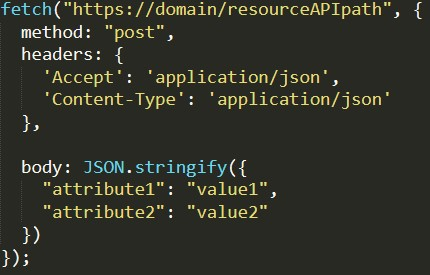
\includegraphics[scale=1.2]{../Img/fetchPOST}
	\caption{Fetch POST API}\label{}
\end{figure}
Once triggered, these functions retrieve the event and put it in the \emph{MessageBody} parameter. The event object is not changed, instead in the user functions which encrypt the password before sending the message to corresponding SQS queue.\\
Example:
\begin{lstlisting}[escapechar=\%]
module.exports.pushUpdateRoleToSQS = (event, context, callback) => {
	const AWS = require(%'%aws-sdk%'%);
	const SQS = new AWS.SQS();
	const stringedEvent = JSON.stringify(event);
	
	const params = {
		MessageBody: stringedEvent,
		QueueUrl: "https://yourDomain/updateRoleQueue"
	};
	
	SQS.sendMessage(params, function(err,data){
		if(err){
			console.log(err);
			callback(null, err);
		}
		else
			callback(null, "Role event pushed to SQS");
	});
};
\end{lstlisting}

\paragraph{CommandOperationAggregate} \Spazio
These functions validate the values of the attributes before storing the event in the \emph{eventStore} and triggered when a new event arrives to the corresponding queue. \\ 
If you have to check for duplicated attributes in the database, the function must be marked \emph{async} because it has to wait for the result of the check operation.\\
Example:
\begin{lstlisting}[escapechar=\%]
module.exports.commandCreateRole = async (event, context, callback) => {
	const utils = require(%'%./utils.js%'%);
	
	const stringedEvent = event.Records[0].body.toString(%'%utf%-%8%'%);
	const eventParsed = JSON.parse(stringedEvent);
	const stringedBody = JSON.stringify(eventParsed);
	const bodyParsed = JSON.parse(stringedBody);
	const check = bodyParsed.body;
	
	const checkNameParams = {
		TableName: %'%role%'%,
		ExpressionAttributeNames:{
			"#rolename": "name"
		},
		ProjectionExpression: "#rolename",
		FilterExpression: "#rolename = :checkname",
		ExpressionAttributeValues: {
			":checkname": check.name
		}
		
	const nameAlreadyExists = await utils.asyncCheckScanDB(checkNameParams);
	
	if((check.roleId == "" || check.name == "" || check.desc == "") || nameAlreadyExists)
		callback(null, "Name already exists or empty attributes");
	else{
		utils.storeEvent("role", "executeCreateRoleQueue", bodyParsed.body);
		callback(null, "Role event stored");
	}
};
\end{lstlisting}

\begin{figure} [H]
\paragraph{Mediator} \Spazio
This function catch the \emph{DynamoDB} event and triggered when a change occurs in a certain table. \\
You have to be careful that the \emph{DynamoDB} events are mapped using the char type attribute value. This is an example: \\

	\centering
	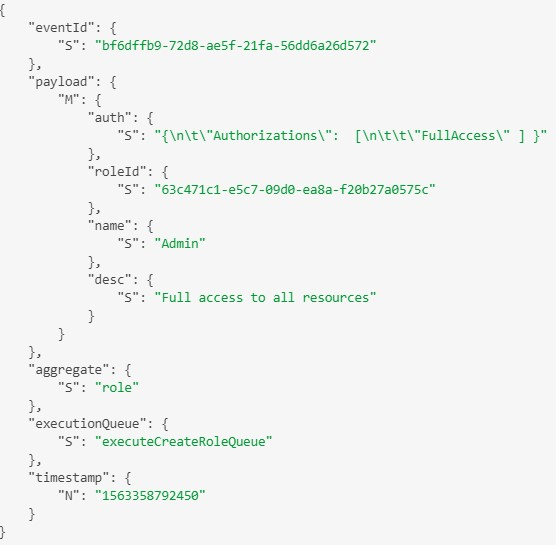
\includegraphics[scale=1.2]{../Img/dynamoEvent}
	\caption{DynamoDB event object}\label{}
\end{figure}

You can use the \emph{"AWS.DynamoDB.Converter"} module to parse a DynamoDB event object.

\begin{figure} [H]
	\centering
	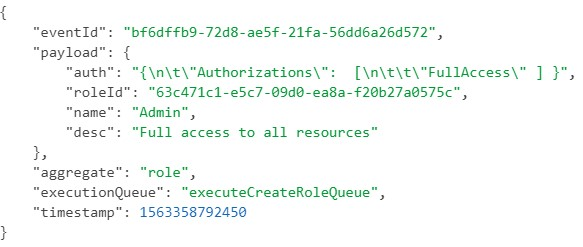
\includegraphics[scale=1.2]{../Img/parsedDynamoEvent}
	\caption{Parsed DynamoDB event object}\label{}
\end{figure}

After that, the mediator retrieves the \emph{executionQueue} parameter from the event object, the payload event passed with the \emph{MessageBody} and then sends the execution message to corresponding SQS queue. 

\paragraph{OperationAggregate} \Spazio
These functions execute a single operation using the event payload and triggered when new event arrives to the corresponding execution queue.\\
Example:
\begin{lstlisting}[escapechar=\%]
module.exports.createRole = async (event, context, callback) => {
	const AWS = require(%'%aws-sdk%'%);
	const dynamoDb = new AWS.DynamoDB.DocumentClient();
	
	const stringedBody = event.Records[0].body.toString(%'%utf%-%8%'%);
	const parsedBody = JSON.parse(stringedBody);
	
	const params = {
		TableName: %'%role%'%,
		Item: parsedBody
	};
	
	await dynamoDb.put(params, (err, data) => {
		if (err){
			console.log(err);
			callback(null, err);
		}
	else
		callback(null, "Role created");
	}).promise();
};
\end{lstlisting}

\paragraph{Recovery} \Spazio
This function allows you to restore the system state starting from a given timestamp by replaying all the events into the \emph{eventStore} table which were stored after that time. \\
Is important to re-execute the events one by one and in the correct order(from the oldest one); for this purpose the recovery function implements a sorting algorithm that retrieves an array of events and sorts them by timestamp, and an \emph{async} function which sends every event to the corresponding execution queue.

\subsubsection{Read mode Lambda functions}
\begin{figure} [H]
\paragraph{ReadOperationAggregate} \Spazio
These functions works in the read side of the architecture; they query the database to retrieve the informations needed without passing throw a SQS queue or a mediator. This kind of events aren't stored into the \emph{eventStore} because they don't change the current system state; this Lambda functions fetch the URL of a GET endpoint using a GET request and listen for a response result. \\

	\centering
	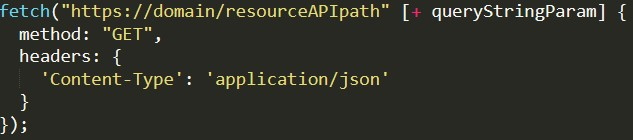
\includegraphics[scale=1.2]{../Img/fetchGET}
	\caption{Fetch GET API}\label{}
\end{figure}
Example:
\begin{lstlisting}[escapechar=\%]
module.exports.getAllRoles = (event, context, callback) => {
	const AWS = require(%'%aws-sdk%'%);
	const dynamoDb = new AWS.DynamoDB.DocumentClient();
	
	const params = {
		TableName: %'%role%'%,
		ExpressionAttributeNames:{
		"#rolename": "name" 
		},
		ProjectionExpression: "#rolename"
	};
	
	dynamoDb.scan(params, (err, data) => {
		const stringedData = JSON.stringify(data);
		if (err){
			console.log(err);
			callback(null, err);
		}
		else{
			if(data.Count == 0){
				console.log("Role not found");
				callback(null, "Role not found");
			}  
			else{
				const response = {
					statusCode: 200,
					headers: {
						%'%Content-Type%'%: %'%application/json%'%,
						%'%Access-Control-Allow-Origin%'%: %'%*%'%,
						%'%Access-Control-Allow-Credentials%'%: true
						},
					body: stringedData
				};
				callback(null, response);
			}      
		}
	});
};
\end{lstlisting}

\subsubsection{CloudWatch Logs}
Amazon CloudWatch is a monitoring and management service built for developers, system operators, site reliability engineers and IT managers. CloudWatch provides you with data and actionable insights to monitor your applications, understand and respond to system-wide performance changes, optimize resource utilization, and get a unified view of operational health. CloudWatch collects monitoring and operational data in the form of logs, metrics, and events. \\
This tool can be very helpful to debug your Lambda functions and to understand what happens to your system.

\subsection{DynamoDB}
Amazon DynamoDB is a fully managed proprietary NoSQL database service that supports key-value and document data structures and is offered by Amazon Web Services.
In this project the DynamoDB instance is used for two purpose: it is used to store events and to keep updated the aggregates views.\\
The tables are the following:
\begin{itemize}
	\item \textbf{eventStore}: to keep track of the occurred events;
	\item \textbf{user}: to store users info;
	\item \textbf{role}: to store roles info;
	\item \textbf{authorization}: to store authorizations info;
	\item \textbf{group}: to store groups info.
\end{itemize}

\subsection{API Gateway}
Amazon API Gateway is a fully managed service that makes it easy for developers to create, publish, maintain, monitor, and secure API at any scale. You can create REST and WebSocket API that act as a “front door” for applications to access data, business logic, or functionality from your backend services.

In this project, API endpoints starting the execution flow of a write mode function through a POST request, pushing a new event into the corresponding queue; in fact you have to provide an API endpoint for each function. On the other side, to query the database you have to reach the endpoint through a GET request to get a result response.

\subsection{Simple Queue Service}
Simple Queue Service(SQS) is a distributed message queuing service introduced by Amazon. It supports programmatic sending of messages via web service applications as a way to communicate over the Internet. SQS is intended to provide a highly scalable hosted message queue that resolves issues arising from the common producer-consumer problem or connectivity between producer and consumer.\\

In this project, for each function you have to use two queues: 
\begin{itemize}
	\item \textbf{OperationAggregateQueue}: this queues receive new events from an API endpoint and trigger the corresponding \emph{commandOperationAggregate} function;
	\item \textbf{ExecuteOperationAggregateQueue}: this queues receive new events from the \emph{mediator} function and trigger the corresponding \emph{operationAggregate} function.
\end{itemize}
